\section{Service Oriented Architecture}
\dbc{Use a more meaningful title that reflect the solution. Also, why are we talking about an initial phase? You can mention that we iterate through several designs. But it's not important to discuss each design in detail unless once design is essential to understand the other design. Ideally, present only the finalized design while adding a single para for each of the previous attempts.}

In the initial phase of WDIAS architecture, it proposed with a \acrfull{soa} as shown in the \ref{fi:proposed_soa}. Mainly it consist of 4 modules, namely:
- Import modules
Import modules are using for integration of data from different source which come in different data formats.
- Export modules
Export modules are using for data dissemination with different format which may required for different type of operations.
- Extension modules
Extension modules are capable of providing the data assimilation functionalities by providing some of key functionalities such as transformation, interpolation and validation. While data assimilation, existing timeseries may be modified or create new timeseries based on the system configurations.
- Adapter module
Adapter module is handling the complexity of integrating different data formats and storing them in the way that easy to search and retrieve.

\begin{figure}[htp]
    \centering
    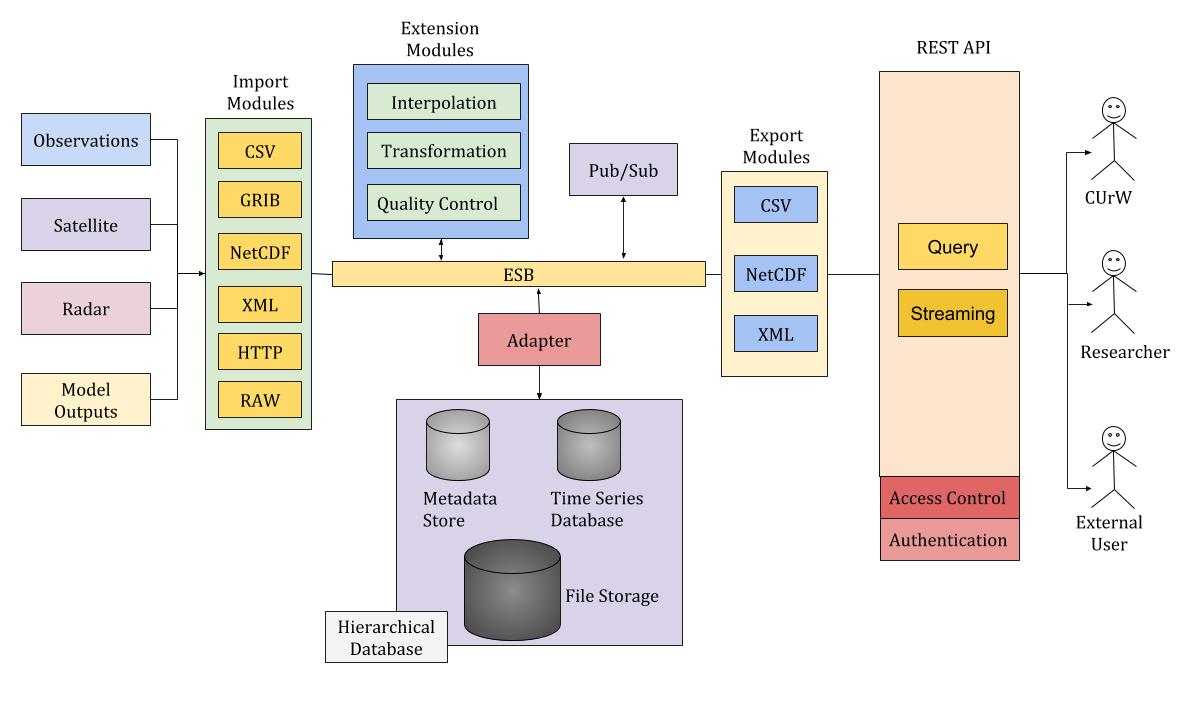
\includegraphics[width=1\textwidth]{soa/soa_v1.jpg}
    \caption{Service oriented architecture of WADIS.}
    \label{fi:proposed_soa}
\end{figure}

- \acrfull{esb}
While implementing a \acrfull{soa}, the \acrfull{esb} can provide capability to integrate different modules, since it is acting as a common layer for all of modules.
By default, \acrshort{esb} provides pub sub capabilities.
\acrshort{esb} mediator can be used to integrate the import, export and extension modules. \acrshort{esb} also support different transportation protocols such as HTTP and Web-Socket etc.

But \acrshort{esb} is not a better solution for data streaming or bulk data processing. Also \acrshort{esb} suffer from single point of failure, since all the messages are going though a common bus.